% !TEX program = xelatex
\documentclass[a4paper,12pt]{article}
\usepackage{graphicx} % Required for inserting images
\usepackage[]{geometry} % Insert size in the [] to define and control the margins on the page
\usepackage{hyperref} % Makes links and table of contents clickable
\hypersetup{colorlinks=true, linkcolor=blue, urlcolor=blue}
% Use this if you want the links to be noticeable and have color blue, the color can be changed
% \usepackage{mathtools} % math tools builds upon amsmath, so only one of them is needed, note that mathtools has all the functions that amsmath has and even more
\usepackage{amsmath,amssymb,amsthm}
\usepackage{tikz}
\usepackage{tikz-cd}
\usepackage{subcaption}
\renewcommand{\qed}{\hfill\blacksquare}
\newcommand{\D}[1]{\Delta #1}
\renewcommand{\a}{\alpha}
\usepackage{tcolorbox}
\tcbuselibrary{theorems}
\usepackage{xcolor}
% \newcommand{\a}{\alpha}
\usepackage{cancel}
\usepackage{float}
\usepackage{enumitem}
\usepackage[T1]{fontenc}
\usepackage{lmodern}
\usepackage{fancyhdr}
\usepackage{titlesec} % For customizing section titles
\usepackage{multicol} % Required for using the multicols environment

\AtBeginDocument{
  \renewcommand\footnoterule{%
    \kern -3pt
    \hbox to \textwidth{\hfill\vrule height 0.4pt width .4\textwidth}
    \kern 2.6pt
  }
}

% Page geometry
\geometry{
  a4paper,
  left=25mm,
  right=25mm,
  top=25mm,
  bottom=25mm
}

\definecolor{myblue}{RGB}{0, 102, 204}
\definecolor{myred}{RGB}{204, 0, 0}
\definecolor{mygreen}{RGB}{0, 153, 76}
\definecolor{lightgray}{gray}{0.95}

\tcbset{
  colback=lightgray, % Background color of the box
  colframe=myblue, % Border color
  coltitle=white, % Title color
  fonttitle=\bfseries, % Title font
  boxrule=0.5mm, % Border thickness
  arc=4mm, % Rounded corners
  auto outer arc,
}

% Custom section headings
\titleformat{\section}
  {\color{myblue}\normalfont\Large\bfseries}
  {\color{myblue}\thesection}{1em}{}

\titleformat{\subsection}
  {\color{myblue}\normalfont\large\bfseries}
  {\color{myblue}\thesubsection}{1em}{}

% Header and footer settings
\pagestyle{fancy}
\fancyhf{}
\fancyhead[L]{\textbf{מתן לבינטוב}} % insert text here
\fancyhead[R]{\textbf{תאוריה כלכלית מיקרו}} % insert text here
\fancyfoot[C]{\thepage}

% Hyperlink settings
\hypersetup{
  colorlinks=true,
  linkcolor=myblue,
  urlcolor=myred,
  citecolor=mygreen,
}

\usepackage{todonotes}
% \renewcommand{\labelitemi}{$\bullet$} # this also works
\setlist[itemize]{label=$\bullet$}
% Define a custom block environment
\newtcolorbox{myblock}[2][]{colback=blue!5!white, colframe=blue!75!black,
    fonttitle=\bfseries, title=#2, #1}

% Define a new tcolorbox environment with automatic numbering
\newtcolorbox[auto counter]{question}[1][]{
  colback=myblue!5!white,  % Background color
  colframe=myblue!75!black,  % Frame color
  fonttitle=\bfseries,  % Title font style
  title=שאלה \thetcbcounter,  % Title format with counter
  #1  % Additional options
}

% Define a new tcolorbox environment with automatic numbering
\newtcolorbox[auto counter]{answer}[1][]{
  colback=mygreen!5!white,  % Background color
  colframe=mygreen!75!black,  % Frame color
  fonttitle=\bfseries,  % Title font style
  title=תשובה \thetcbcounter,  % Title format with counter
  #1  % Additional options
}

% \theoremstyle{plain}% from `amsthm' 
% \newtheorem{lem}{Lemma}% from `amsthm'
\newtcolorbox[auto counter]{remark}[1][]{colback=yellow!5!white, colframe=yellow!75!black, fonttitle=\bfseries, title=הערה  , #1}

% Define a new tcolorbox environment for proofs
\newtcolorbox[auto counter]{Proof}[1][]{colback=mygreen!5!white, colframe=mygreen!75!black, fonttitle=\bfseries, title=הוכחה  , #1}

% Define a new tcolorbox environment for theorems
\newtcolorbox[auto counter]{theorem*}[1][]{colback=myblue!5!white, colframe=myblue!75!black, fonttitle=\bfseries, title=משפט  , #1}

% Define a new tcolorbox environment for definitions
\newtcolorbox[auto counter]{definition}[1][]{colback=red!5!white, colframe=red!75!black, fonttitle=\bfseries, title=הגדרה  , #1}


% Define a new tcolorbox environment for conjectures
\newtcolorbox[auto counter]{conjecture}[1][]{
  colback=orange!5!white,  % Background color
  colframe=orange!75!black,  % Frame color
  fonttitle=\bfseries,  % Title font style
  title=השערה ,  % Title format with counter
  #1  % Additional options
}

% \renewenvironment{proof}[1][Proof.]{\textbf{#1} }{\ \rule{0.5em}{0.5em}}
\newtheorem{theorem}{משפט}
% \newtheorem*{theorem*}{משפט}
\newtheorem{notation}{כתיב}
\newtheorem{claim}{טענה}
\newtheorem{cor}{Corollary}
% \newtheorem{conj}{Conjecture}
\newtheorem{fact}{עובדה}
\newtheorem{lemma}{למה}
\newtheorem{condition}{תנאי}
% \newtheorem{definition}{הגדרה}
\newtheorem{obs}{Observation}
\newtheorem{proposition}{Proposition}
\newtheorem{assumption}{הנחה}
\newtheorem{defn}{Definition}
\newtheorem{example}{Example}
\newtheorem{corollary}{טענת עזר}
% \newtheorem{question}{Question}
\newtheorem{problem}{Problem}
% \newtheorem{remark}{Remark}
\newtheorem{diagram}{}
% \newcommand{\ML}[1]{\todo[color=yellow!20,author=\textbf{מתן},inline]{\small #1}}
% \newcommand{\YS}[1]{\todo[color=blue!20,author=\textbf{יובל},inline]{\small #1}}
% ============================================================ %
% HEBREW support via polyglossia %
% ============================================================ %
\usepackage{polyglossia}
\defaultfontfeatures{Mapping=tex-text, Scale=MatchLowercase}
\setdefaultlanguage{hebrew}
\setotherlanguage{english}
\newfontfamily\hebrewfont[Script=Hebrew]{David CLM}
% Use \begin{hebrew} block of text \end{hebrew} for paragraphs.
% Use \texthebrew{ } and \textenglish{ } for short texts.
% ============================================================ %
\newcommand{\te}[1]{\textenglish{#1}}
\usepackage{bidi} % we use bidi for Right-To-Left (RTL) writing
\title{הוכחות \footnote{התרגילים והגדרות נלקחו מתוך \te{Hammack, R (2013). Book of Proof}}}
\author{מתן לבינטוב}
\date{}
% Begin of Document ---------------------------------------- %
\begin{document}
\begin{RTL}
\maketitle
\begin{abstract}
זהו התרגול הראשון בקורס תאוריה כלכלית מיקרו אשר נועד לספק בסיס להוכחות פורמליות, דבר שלא ממש פגשת עד עכשיו בתואר הראשון. לא כל הגדרה במסמך הזה תהיה מוגדרת בצורה המדויקת ביותר מתוך אילוצי זמן. כל האי דיוקים במסמך זה נעשו מתוך כוונה לפשט את הרעיונות שמוצגים כאן.
\end{abstract}

\newpage
\tableofcontents
\newpage

\section{הגדרות}

\subsection{\te{Theorem}}
משפט / טענה אשר נכון והוכח שהוא נכון, לדוגמה :
\begin{theorem*}
תהי $f$ גזירה ב $(a,b)$ וניקח $c \in (a,b)$ כך ש $f(c)$ הוא מקסימום או מינימום של הפונקציה בקטע $(a,b)$ אזי $f'(c) = 0$.
\end{theorem*}

% \begin{theorem*}
% אם $\displaystyle \sum_{k=1}^{\infty} a_k$ היא סדרה מתכנסת אז $\displaystyle \lim_{k \to \infty} a_k = 0$.
% \end{theorem*}

\subsection{\te{Proposition}}
משפט נכון בדיוק כמו \te{Theorem}, הבדל נובע בדרך כלל בחשיבות

\subsection{\te{Lemma}}
טענת עזר, משפט שמשמש להוכיח משפט אחר גדול יותר / חשוב יותר.

\subsection{\te{Corollary}}
משפט שנובע מיידית מתוצאות / משפטים קודמים.


\section{קבוצות וקבוצות המספרים}
\subsection{המספרים הטבעים}
מסומנים $\mathbb{N}$, וכוללים את כל המספרים החיובים חוץ מ0, 
$$
\{1,2,3,4,5,6,7,8, \ldots\} = \mathbb{N}
$$

\subsection{המספרים השלמים}
מסומנים $\mathbb{Z}$, וכוללים את כל המספרים השלמים כולל 0,
$$
\{ \ldots, -3, -2, -1, 0, 1, 2, 3, \ldots \} = \mathbb{Z}
$$
או לחילופין ניתן גם להגדיר אותם כך,
$$
\mathbb{Z} = \{n | n \in \mathbb{N}\} \cup \{0\} \cup \{-n | n \in \mathbb{N}\}
$$

\subsection{המספרים הרציונליים} 
מסומנים ב-$\mathbb{Q}$, וכוללים את כל המספרים המתקבלים כמנה של שני מספרים שלמים, לדוגמה $\frac{1}{2}$, $\frac{3}{4}$, $\frac{5}{3}$ וכו'. פורמלית,

$$
\mathbb{Q} = \left\{ \frac{m}{n} \ \big | \  m,n \in \mathbb{Z}, n \neq 0 \right\}
$$

\subsection{הממשיים}
מסומנים ב-$\mathbb{R}$, והם כל המספרים בציר המספרים, כולל את הרציונלים וגם את הלא רציונלים, ניתן להגדיר אותם פורמלית בעזרת סדרה מתכנסת של $\mathbb{Q}$ אך לא נעשה זאת פה, מוזמנים לבדוק באינטרנט את הגדרה הפורמלית. כן ניתן דוגמאות למספרים ממשיים,
$$
e, \pi, \sqrt{2}, \sqrt{3}, \sqrt{5}, \sqrt{7}, 2 , 1 , 0, -1, -2, -\pi, -e \in \mathbb{R}
$$
נשים לב שאפשר לבנות את קבוצת כל המספרים הלא רציונלים על ידי לקיחת $\mathbb{R}$ ומחיקה של $\mathbb{Q}$ ממנו, נסמן את הקבוצה הזו ב-$\mathbb{R} \setminus \mathbb{Q}$.

\begin{remark}
נשים לב שיש קשר בין כל הקבוצות שציינו, לפי הסדר שציינו אותם, כל קבוצה מוכלת בקבוצה אשר באה אחריה. בצורה פורמלית אפשר לכתוב זאת ככה,
$$
\mathbb{N} \subset \mathbb{Z} \subset \mathbb{Q} \subset \mathbb{R}
$$
וכמובן שיש גם איור יפה שמראה את הקשרים הללו.
\begin{figure}[H]
  \centering
  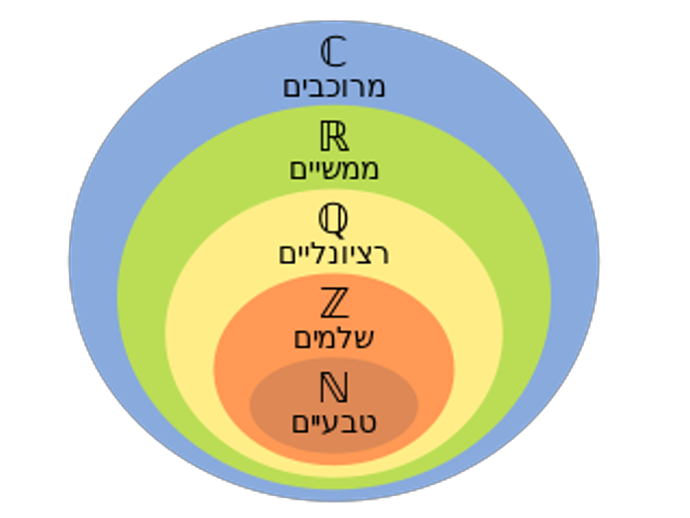
\includegraphics[width=0.8\textwidth]{figures/sets.png}
  \caption{קבוצות המספרים}
  \label{fig:number_sets}
\end{figure}
\end{remark}


\newpage

\section{הוכחות}
נעבור על השיטות המרכזיות להוכחת משפטים, ונציג כמה דוגמאות לכל סוג של הוכחה.
אך קודם עלינו להגדיר 2 הגדרות אשר נשתמש בהם בהוכחות.

\begin{definition}
מספר זוגי. מספר $n$ הוא זוגי אם קיים $k \in \mathbb{Z}$ כך ש $n = 2k$.
\end{definition}

\begin{definition}
מספר אי-זוגי. מספר $n$ הוא אי-זוגי אם קיים $k \in \mathbb{Z}$ כך ש $n = 2k + 1$.
\end{definition}

\subsection{הוכחה ישירה}
אם א' אז ב' או לחלופין $P \implies Q$. מה שזה אומר זה שאם $P$ נכון / מתקיים אז הוא גורר / מקיים גם את $Q$. בהוכחה ישירה מהסוג הזה של טענות נניח ש $P$ נכון / מתקיים ונוכיח שגם $Q$ נכון / מתקיים.

\begin{theorem*}
אם $x$ אי-זוגי אזי $x^2$ אי-זוגי.
\end{theorem*}

\begin{Proof}
נניח ש $x$ הוא אי-זוגי, לפי הגדרה של מספר אי-זוגי, 
$$
x = 2k + 1
$$
ל - $k$ מסוים ב $\mathbb{Z}$. לכן ,
$$
x^2 = (2k + 1)^2 = 4k^2 + 4k + 1 = 2(2k^2 + 2k) + 1 = 2m + 1
$$
כאשר $m = 2k^2 + 2k$ הוא מספר שלם, ולכן $x^2$ אי-זוגי. $\qed$
\end{Proof}

\subsection{הוכחה בעזרת \te{Contrapositive}}
בלוגיקה, המשפט $P \implies Q$ שקול לוגית למשפט $\sim Q \implies \sim P$. כלומר המשפט א' גורר ב' זהה למשפט לא ב' גורר לא א'. ניתן להוכיח את השקילות הזאת על ידי טבלת אמת אך לא נעשה זאת כאן ונקבל את השקילות כנכונה בלי הוכחה. בדומה להוכחה הישירה, על מנת להוכיח משפט בשיטה הזו, נניח שלא $Q$ נכון ונוכיח שלא $P$ נכון.
\begin{theorem*}
לכל $x \in \mathbb{Z}$ אם $x^2 - 6x + 5$ זוגי, אזי $x$ אי-זוגי.
\end{theorem*}

\begin{Proof}
נניח ש $x$ הוא לא אי-זוגי, כלומר $x$ זוגי. לפי הגדרה של מספר זוגי,
$$
\exists k \in \mathbb{Z}, \ x = 2k
$$
לכן, 
$$
x^2 - 6x + 5 = (2k)^2 - 6(2k) + 5 = 4k^2 - 12k + 5 = 2(2k^2 - 6k) + 5 = 2m + 5
$$
אפשר לראות שאנחנו מאוד קרובים אבל זאת לא בדיוק הגדרה של מספר אי-זוגי, מה שאפשר לעשות זה לפרק את $5$ ל $4+1$. נחזור לשוויון האמצעי,
$$
4k^2 - 12k + 4 + 1 = 2(2k^2 - 6k + 2) + 1 = 2a + 1
$$
כאשר $a = 2k^2 - 6k + 2$ הוא מספר שלם, ולכן $x^2 - 6x + 5$ אי-זוגי לפי הגדרה. $\qed$
\end{Proof}

\subsection{הוכחה בשלילה}
הוכחה בשלילה הולכת ככה, תהי טענה $P$, אם כתוצאה מהנחה , $\sim P \implies C \wedge \sim C$ כלומר, הנחנו שהטענה לא נכונה וקיבלנו שטענה $C$ היא גם נכונה וגם לא נכונה באותו הזמן, כלומר סתירה לוגית. מכך הנחה שלנו ש $\sim P$ היא לא נכונה ולכן $P$ נכונה. גם פה ניתן לנתח את השקילות הלוגית של השיטה הזו על ידי טבלת אמת אך נקבל את השקילות כנכונה בלי הוכחה.

\begin{remark}
  בהוכחות מהסוג של הוכחה בשלילה מקובל להתחיל את ההוכחה ב "נניח בשלילה ש...." \te{(Assume for the sake of contradiction that... / Assume towards a contradiction that...)}.
\end{remark}
בשביל הדוגמה שלנו לסוג ההוכחה הזה נצטרך עוד הגדרה,
\begin{definition}
מספר $x$ הוא רציונלי (כלומר $x \in \mathbb{Q}$) אם קיימים $m,n \in \mathbb{Z}$ כך ש $x = \frac{m}{n}$ ו $n \neq 0$. מספר $x$ הוא לא רציונלי אם לא קיימים $m,n$ כאלו.
\end{definition}

\begin{theorem*}
$\sqrt{2}$ אינו רציונלי. ($\sqrt{2} \notin \mathbb{Q}$)
\end{theorem*}

\begin{Proof}
נניח בשלילה ש - $\sqrt{2} \in \mathbb{Q}$, כלומר $\exists m,n \in \mathbb{Z}$ כך ש $\sqrt{2} = \frac{m}{n}$ ונוסיף לכך ש - $\sqrt{2}$ מוצג בגרסה המצומצמת ביותר שלו. מכאן,
\begin{align}
\sqrt{2} &= \frac{m}{n}  \\
2 &= \frac{m^2}{n^2}  \\
2n^2 &= m^2 
\end{align}
נשים לב שקיבלנו ש $m^2$ הוא מספר זוגי לפי הגדרה. ניזכר שקודם לכן הוכחנו את הטענה שאם $x$ הוא אי-זוגי אזי $x^2$ הוא גם אי-זוגי, ללא עבודה והוכחה נוספת ניתן להפוך את המשפט (\te{Counterpositive}) ולקבל את הטענה הבאה שהיא שקולה לוגית ואין צורך להוכיח אותה כי כבר עשינו זאת.

אם $x^2$ זוגי אזי $x$ זוגי.
מכך נובע ש $m$ זוגי, כלומר קיים $k \in \mathbb{Z}$ כך שניתן לכתוב את $m$ בצורה הבאה $m = 2k$ . נציב את זה במשוואה מספר 3,
\begin{align}
2n^2 &= (2k)^2 = 4k^2 \\
n^2 &= 2k^2
\end{align}
עם טיעון זהה למה שטענו מקודם קיבלנו שגם $n$ זוגי, אבל אם המונה וגם המכנה זוגיים אז קיים מכנה משותף שניתן לצמצם בו את המנה (2) וזאת סתירה להנחה ש $\sqrt{2}$ מוצג בגרסה המצומצמת שלו. $\implies \impliedby$ 

$\qed$
\end{Proof}


\subsection{טענות מסוג אם ורק אם / \te{if and only if (iff)}}
במהלך הקורס תפגשו טענות מהסוג הבא,
$$
P \iff Q
$$
בפועל זה אומר ששני הטענות הבאות נכונות,
\begin{enumerate}
  \item $P \implies Q$
  \item $Q \implies P$
\end{enumerate}
כלומר, יש פה טענה מאוד חזקה, אם $P$ נכון אז גם $Q$ ואם $Q$ נכון אז גם $P$.
איך מוכיחים טענות כאלו? מאוד פשוט, מתייחסים אליהם כאל 2 טענות נפרדות ומוכיחים כל כיוון בנפרד, פעם אחת מניחים $P$ ומוכיחים שממנו נובע $Q$ ופעם השנייה מניחים ש $Q$ נכון ומוכיחים שממנו נובע $P$.

\begin{remark}
  בדרך כלל בהוכחות מסוג אם ורק אם נהוג לסמן כל כיוון בסימון $\implies$ ו $\impliedby$.
\end{remark}
\begin{theorem*}
  המספר $x$ הוא אי זוגי אם ורק אם $x^2$ אי זוגי.
\end{theorem*}

\begin{Proof}
  $\impliedby$\\
  נניח ש $x$ הוא אי זוגי, כלומר, לכן ניתן לכתוב אותו כך $x = 2k + 1$ עבור $k \in \mathbb{Z}$. נציב את זה ב $x^2$,
  \begin{align}
    x^2 &= (2k + 1)^2 = 4k^2 + 4k + 1 = 2(2k^2 + 2k) + 1 = 2m + 1
  \end{align}
  ולכן $x^2$ אי זוגי.\\

  $\implies$\\

  להניח ש $x^2$ הוא אי זוגי ולהוכיח שזה גורר $x$ הוא גם אי-זוגי נשמע לא נוח, לכן נוכיח את ה \te{Counterpositive} שלה, כלומר נוכיח את המשפט הבא : אם $x$ הוא זוגי אז $x^2$ גם זוגי. נניח ש $x$ הוא זוגי, כלומר $x = 2k$ עבור $k \in \mathbb{Z}$, נציב את זה ב $x^2$,
$$
x^2 = (2k)^2 = 4k^2 = 2(2k^2)
$$
מכך נובע ש $x^2$ זוגי ולכן נקבל את הטענה המקורית כנכונה. $\qed$
\end{Proof}

\subsection{הפרכה / \te{Disproving}}
לא כל הטענות שתפגשו הן נכונות ולכן נצטרך להפריך אותן, כעת נראה איך עושים זאת.

\begin{conjecture}
 לכל מספר $n \in \mathbb{Z}$ המספר $f(n) = n^2 - n + 11$ הוא מספר ראשוני.
\end{conjecture}
אם נתחיל להציב מספרים בשביל להבין את הבעיה נתחיל לחשוב שהטענה נכונה אבל נשים לב שב - $n = 11$ המספר שמתקבל הינו $f(11) = 11^2 - 11 + 11 = 121$. כלומר מצאנו מספר שאינו ראשוני ולכן הטענה לא נכונה.

\begin{remark}
  נשים לב שזה היה יחסית פשוט, הטענה השתמשה בכמת "לכל" ולכן על מנת להפריך אותה מספיק מאיתנו למצוא דוגמה נגדית אחת. אך מה קורה אם במקום שהטענה תדרוש "לכל" מספר היא תדרוש  ש"קיים" מספר? איך מפריכים טענה כזאת?
\end{remark}

\begin{conjecture}
  קיים $x \in \mathbb{R}$ כך ש $x^4 < x < x^2$.
\end{conjecture}
עם קצת משחקי הצבה ואפילו קצת הצבות חכמות אנחנו מבינים מאוד מהר שיש פה בעיה ואולי הטענה לא נכונה. על מנת להוכיח שהטענה לא נכונה, אפשר להוכיח שהופכי שלה הוא נכון. מה ההופכי של הטענה?

\begin{theorem*}
  \textbf{לכל} $x \in \mathbb{R}$ לא מתקיים $x^4 < x < x^2$.
\end{theorem*}
\begin{Proof}
  נניח בשלילה שכן מתקיים $x$ כך ש $x^4 < x < x^2$.  קל לראות שבגלל החיוביות של $x^4$ והעובדה שמדובר באי-שיווינות חזקים $x$ חייב להיות מספר חיובי ממש $(x > 0)$. לכן ניתן לחלק את כל החלקים ב - $x$, 
  \begin{align*}
    x^3 &< 1 < x \\
    \left(x-1\right)\left(x^2 + x + 1\right) &< 0 < x - 1 \\
    x^2 + x + 1 & < 0 < 1
  \end{align*}
  נשים לב לכמה דברים, קודם כל חילוק כל החלקים ב - $x-1$ בין השורה השנייה לשלישית לא גורר היפוך של הא''ש בגלל שהא''ש הימיני של שורה 2 אומר ש $x - 1 > 0$. עכשיו שימו לב לתוצאה המעניינת שקיבלנו קודם לכן הגענו למסקנה ש $x > 0$ אבל אם נסתכל על הא''ש האחרון אנחנו קיבלנו שסכום של 3 איברים חיובים $(x^2, x, 1)$ הוא מספר שלילי ממש (קטן מ0) וזאת סתירה. $\implies \impliedby$ \\
  לכן  \textbf{לכל} $x \in \mathbb{R}$ לא מתקיים $x^4 < x < x^2$. $\qed$

\end{Proof}
היות והצלחנו להוכיח את השלילה של השערה שלנו, ההשערה לא נכונה.

% \section{גודל של קבוצות / \te{Cardinality}} 
% ישנו רעיון חשוב מאוד שעוד לא דיברנו עליו בנוגע לקבוצות והוא גודל הקבוצה. נניח שיש לנו 2 קבוצות $A$ ו $B$, איך יודעים איזו מהקבוצות גדולה יותר? (השאלה היא אפילו מעניינת יותר כאשר מדובר בקבוצות אינסופיות) בפרט איך מכמתים גודל של קבוצה? נתחיל בפשוט, נניח שיש לנו 2 קבוצות סופיות,
% $$
% A = \{1,2,3,4,5\} \quad B = \{6,7,8,9,10\}
% $$
% אפשר לראות שאפשר לקחת כל איבר בקבוצה $A$ ולזווג אותו עם איבר בקבוצה $B$ כך שכל איבר בקבוצה $B$ מזווג עם איבר מקבוצה $A$ והוא מזווג עם רק איבר אחד. לדוגמה, 
% $$
% 1 \longleftrightarrow 6, \quad 2 \longleftrightarrow 7, \quad 3 \longleftrightarrow 8, \quad 4 \longleftrightarrow 9, \quad 5 \longleftrightarrow 10
% $$
% קל לטעון כאן שהקבוצות $A$ ו$B$ הן בעלות גודל זהה הרי הצלחנו למפות כל איבר ב $A$ ל$B$ בלי להשמית איברים מ$B$ ומבלי למפות יותר מאיבר אחד ב$A$ לאיבר ב$B$.
% כעת נגדיר את מה שעשינו פורמלית,
% \begin{definition}
%   פונקציה $f: A \to B$ היא חד חד ערכית (חח''ע) או 1-1 אם : 
%   $$
%   f(x_1) = f(x_2) \implies x_1 = x_2.
%   $$
%   או לחילופין, 
%   $$
%   x_1 \neq x_2 \implies f(x_1) \neq f(x_2).
%   $$
% \end{definition}
% במילים, כל איבר ב $A$ מצביע / מזווג רק לאיבר אחד ב $B$.
% \begin{definition}
%   פונקציה $f: A \to B$ נקראת על אם :
%   $$
%   \forall b \in B,  \exists a \in A \implies f(a) = b
%   $$
% \end{definition}
% אינטואיבית, פונקציה היא על אם לכל איבר בקבוצה $B$ קיים איבר בקבוצה $A$ כך שהוא מצביע עליו או מזווג איתו, כלומר כל איבר ב $B$ מוצבע או מזווג עם לפחות איבר אחד (יכול להיות יותר מ1) ב - $A$. 

% \begin{definition}
%   פונקציה $f: A \to B$ נקראת חד חד ערכית ועל (\te{Bijective}) אם היא חח''ע ועל.
% \end{definition}

% נסמן את גודל (עוצמה) קבוצה $A$ ב $|A|$.

% \begin{definition}
%   הקבוצה $A$ והקבוצה $B$ בעלות עוצמה (גודל) זהה אם קיימת פונקציה חד חד ערכית ועל מ $A$ ל $B$ $(f : A \to B)$.\\
%   ונסמן זאת ב $|A| = |B|$.
% \end{definition}

% סימונים נוספים,

% \begin{itemize}
%   \item אם $A = \emptyset$ אז $|A| = 0$.
%   \item אם $A = \{1,2,3,4,\dots, n\}$ אזי $|A| = n$.
%   \item אם קיימת פונקציה חד חד ערכית מ $A$ ל $B$ אזי $|A| \leq |B|$. (זאת משום שלא בהכרח כל האיברים ב $B$ מזווגים ולכן $B$ יכולה להיות גדולה יותר מ $A$.)
%   \item אם קיימת פונקציה על מ $A$ ל $B$ אזי $|A| \geq |B|$. (זאת משום שכל איבר ב $B$ מזווג / ממופה אבל יכול להיות שיש כמה איברים ב$A$ שמצביעים על אותו איבר ב$B$.)
% \end{itemize}
% ונסיים בהגדרה העיקרית שלנו,
% \begin{definition}
%   אם לקבוצה $A$ אותה עוצמה כמו ל $\mathbb{N}$, כלומר $|A| = |\mathbb{N}|$ אז $A$ נקראת קבוצה בת מנייה אינסופית (\te{Countably Infinite}). \\
%   אם קבוצה $A$ היא סופית אז היא נקראת בת מנייה סופית.
% \end{definition}
% לסיכום, קבוצה $A$ נקראת בת מנייה אם העוצמה שלה קטנה או שווה לעוצמה של המספרים הטבעים ($|A| \leq |\mathbb{N}|$), אחרת קבוצה $A$ לא בת מנייה.

% דוגמאות לקבוצות בנות מנייה,
% \begin{multicols}{2}
% \begin{itemize}
%   \item $\mathbb{Z}$
%   \item $\mathbb{Q}$
%   \item $\mathbb{N} \times \mathbb{N}$
%   \item $\mathbb{Z} \times \mathbb{Z}$
% \end{itemize}
% \end{multicols}

% \begin{theorem*}
%   לא קיימת פונקציה חד חד ערכית ועל מהטבעים ($\mathbb{N}$) לממשיים ($\mathbb{R}$), כלומר $\mathbb{R}$ לא בת מנייה!
% \end{theorem*}
% במידה וזה מעניין אותכם ניתן למצוא הוכחה למשפט זה בספרים רבים וגם באינטרנט.

\end{RTL}
\end{document}